\documentclass[11pt]{article}

% ---------------------------------------------------------------------------
%  The ZETA test, explained -- a plain-language companion to the HGF guide.
%  Matches the visual style of Hierarchical_Gaussian_Filter_explained.pdf:
%  teal section headings, teal "key insight" and rust "deeper insight"
%  callout boxes, a TikZ flow diagram, pgfplots figures, a symbol glossary.
% ---------------------------------------------------------------------------

\usepackage[a4paper,left=3cm,right=3cm,top=2.6cm,bottom=2.6cm]{geometry}
\usepackage{lmodern}
\usepackage[T1]{fontenc}
\usepackage{amsmath,amssymb}
\usepackage{microtype}
\usepackage{booktabs}
\usepackage{xcolor}
\usepackage{titlesec}
\usepackage{tcolorbox}
\tcbuselibrary{skins}
\usepackage{tikz}
\usepackage{pgfplots}
\pgfplotsset{compat=1.18}
\usetikzlibrary{arrows.meta,positioning,shapes.geometric}
\usepackage{enumitem}
\setlist{itemsep=2pt,topsep=4pt}

% ---- colours (matched to the HGF document) --------------------------------
\definecolor{deepteal}{RGB}{13,95,102}
\definecolor{tealbg}{RGB}{233,242,242}
\definecolor{rust}{RGB}{180,84,40}
\definecolor{rustbg}{RGB}{250,238,228}

% ---- section heading style ------------------------------------------------
\titleformat{\section}{\Large\bfseries\color{deepteal}}{\thesection}{0.7em}{}
\titleformat{\subsection}{\large\bfseries\color{deepteal}}{\thesubsection}{0.6em}{}
\titlespacing*{\section}{0pt}{1.6em}{0.6em}

% ---- callout boxes --------------------------------------------------------
\newtcolorbox{keybox}{
  enhanced,
  colback=tealbg, colframe=tealbg, arc=1.6mm, boxrule=0pt,
  borderline north={2.4mm}{0mm}{deepteal},
  left=4mm,right=4mm,top=3.5mm,bottom=3.5mm,
}
\newtcolorbox{deepbox}{
  enhanced,
  colback=rustbg, colframe=rustbg, arc=1.6mm, boxrule=0pt,
  borderline north={2.4mm}{0mm}{rust},
  left=4mm,right=4mm,top=3.5mm,bottom=3.5mm,
}

% ---- title ----------------------------------------------------------------
\newcommand{\headerrule}{\noindent\textcolor{deepteal}{\rule{\linewidth}{0.6pt}}}

\begin{document}
\thispagestyle{empty}

\begin{center}
  {\Huge\bfseries The ZETA Test\par}
  \vspace{4pt}
  {\large\itshape A plain-language guide to how it works\par}
  \vspace{10pt}
  \textcolor{deepteal}{\rule{0.45\linewidth}{0.5pt}}
\end{center}
\vspace{6pt}

\noindent
This guide explains the \textbf{ZETA test} (\emph{Zenith of Event-based
Time-locked Anomalies}), a way to decide whether a neuron responds to an event
without ever choosing a time bin or a response window. The goal here is
understanding, not brevity: every symbol is introduced in words before it
appears in a formula, and every formula is followed by what it is really doing.
We build up from the problem, through the one curve at the heart of the method,
to the number it produces and what that number does --- and does not --- mean.

% ===========================================================================
\section{What problem does ZETA solve?}

You have recorded a neuron and you have a list of times at which some event
happened --- a cue, a reward, a movement. You want to answer one question:
\emph{does this neuron's firing change around that event?} It sounds simple,
but the standard way of answering it hides two arbitrary choices.

The usual recipe is to build a \textbf{PSTH}: chop the time around the event
into bins, count spikes in each bin across trials, and run a $t$-test or ANOVA
comparing ``after'' to ``before''. To do that you must pick

\begin{itemize}
  \item a \textbf{bin width} --- too wide and a brief response is averaged
        away; too narrow and noise swamps it; and
  \item a \textbf{response window} --- the stretch of time you decide, in
        advance, the response should live in.
\end{itemize}

Both choices change the answer, and testing many bins reopens the
multiple-comparisons problem you were trying to avoid. A sharp, transient
response and a slow, sustained one need different bins to be seen at all --- so
a single fixed choice is always wrong for some neurons.

\begin{keybox}
ZETA throws away both choices. It works directly from the raw spike times and
asks a single binning-free question: \emph{is the timing of the spikes after
the event anything other than what a constant, unchanging firing rate would
produce?} No bin width, no response window, no arbitrary cut-off.
\end{keybox}

% ===========================================================================
\section{The core picture: one curve, end to end}

Everything in ZETA flows through a single object --- the cumulative spike
curve --- and then collapses to one number. The whole pipeline is five steps:

\begin{center}
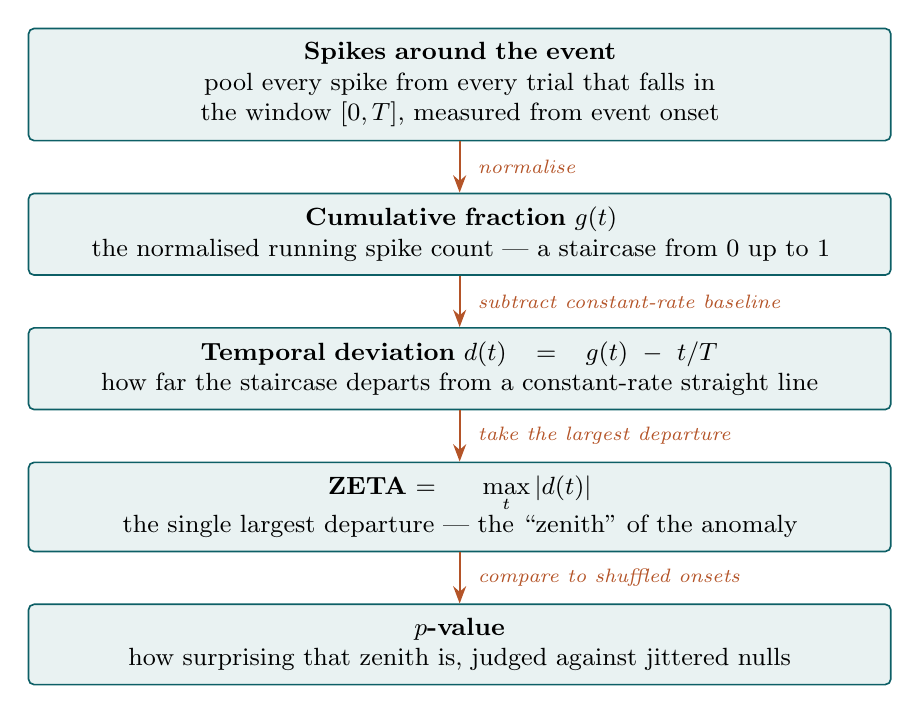
\begin{tikzpicture}[
  box/.style={draw=deepteal, line width=0.6pt, rounded corners=2pt,
              fill=tealbg, text width=10.6cm, align=center,
              inner sep=5pt, font=\small},
  arr/.style={-{Stealth[length=2.2mm]}, rust, line width=0.8pt},
  lbl/.style={font=\scriptsize\itshape, rust, midway, right=1mm},
  node distance=6.5mm,
]
\node[box] (a) {\textbf{Spikes around the event}\\
  pool every spike from every trial that falls in the window $[0,T]$,
  measured from event onset};
\node[box, below=of a] (b) {\textbf{Cumulative fraction} $g(t)$\\
  the normalised running spike count --- a staircase from $0$ up to $1$};
\node[box, below=of b] (c) {\textbf{Temporal deviation} $d(t)=g(t)-t/T$\\
  how far the staircase departs from a constant-rate straight line};
\node[box, below=of c] (d) {\textbf{ZETA} $=\displaystyle\max_t |d(t)|$\\
  the single largest departure --- the ``zenith'' of the anomaly};
\node[box, below=of d] (e) {\textbf{$p$-value}\\
  how surprising that zenith is, judged against jittered nulls};

\draw[arr] (a) -- (b) node[lbl]{normalise};
\draw[arr] (b) -- (c) node[lbl]{subtract constant-rate baseline};
\draw[arr] (c) -- (d) node[lbl]{take the largest departure};
\draw[arr] (d) -- (e) node[lbl]{compare to shuffled onsets};
\end{tikzpicture}
\end{center}

\noindent
The rest of this guide walks down that ladder one rung at a time.

% ===========================================================================
\section{From spikes to a cumulative fraction}

Start at the top of the ladder. Take every event onset, and collect every spike
that lands within a window of length $T$ after it (the parameter
\texttt{dblUseMaxDur} in the code; $T=2$\,s in our analyses). Measure each spike
time \emph{relative to its event}, and pool them all into one long list,
sorted in time: $t_1 \le t_2 \le \dots \le t_n$, where $n$ is the total number
of spikes across all trials.

Now define the \textbf{cumulative spike fraction}: at any time $t$, what share
of all the spikes have happened by then?

\[
  g(t) \;=\; \frac{\#\{\text{spikes with time} \le t\}}{n}.
\]

Each spike steps the curve up by exactly $1/n$, so $g$ climbs as a staircase
from $g(0)=0$ to $g(T)=1$. This is simply the empirical cumulative
distribution of the spike times.

\begin{keybox}
Dividing by the total count $n$ is the crucial move. It strips out the neuron's
overall firing \emph{rate}: a $30$\,Hz cell and a $3$\,Hz cell both produce a
curve running from $0$ to $1$. What survives is the \emph{temporal shape} ---
\emph{when} the spikes arrive, not how many. That is what makes ZETA scale-free
and bin-free. (This is exactly why the curve always ends at $1$.)
\end{keybox}

% ===========================================================================
\section{The constant-rate baseline, and the deviation}

What would $g(t)$ look like for a neuron that \emph{ignores} the event? If the
firing rate were constant, spikes would be spread uniformly across the window,
and an equal fraction would accumulate in each equal slice of time. The
cumulative fraction would then be a straight diagonal line:

\[
  L(t) \;=\; \frac{t}{T},
\]

running from $(0,0)$ to $(T,1)$. This is the null shape --- ``no time-locking''
drawn as a curve. The \textbf{temporal deviation} is the gap between what the
neuron actually did and this flat-rate expectation:

\[
  d(t) \;=\; g(t) - L(t)
  \qquad\text{(then shifted to have zero mean).}
\]

A neuron that bursts just after the event piles up spikes early, so its
staircase bows \emph{above} the diagonal and $d(t)$ is positive there. A neuron
that goes silent and fires late bows below, and $d(t)$ is negative. A neuron
that truly ignores the event hugs the diagonal and $d(t)$ stays near zero.

\begin{center}
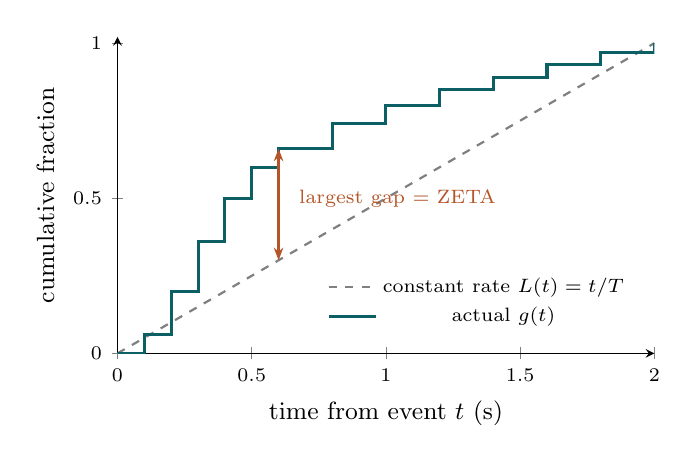
\begin{tikzpicture}
\begin{axis}[
  width=8.4cm, height=5.6cm,
  xlabel={\small time from event $t$ (s)},
  ylabel={\small cumulative fraction},
  xmin=0, xmax=2, ymin=0, ymax=1.02,
  xtick={0,0.5,1,1.5,2}, ytick={0,0.5,1},
  tick label style={font=\scriptsize},
  label style={font=\scriptsize},
  legend style={font=\scriptsize, at={(0.97,0.05)}, anchor=south east,
                draw=none, fill=none},
  axis lines=left,
]
% constant-rate diagonal
\addplot[gray, dashed, line width=0.8pt] coordinates {(0,0) (2,1)};
\addlegendentry{constant rate $L(t)=t/T$}
% real cumulative staircase (illustrative: early burst)
\addplot[deepteal, line width=1.1pt, const plot] coordinates {
  (0,0) (0.1,0.06) (0.2,0.20) (0.3,0.36) (0.4,0.50) (0.5,0.60)
  (0.6,0.66) (0.8,0.74) (1.0,0.80) (1.2,0.85) (1.4,0.89)
  (1.6,0.93) (1.8,0.97) (2.0,1.0)};
\addlegendentry{actual $g(t)$}
% the gap = ZETA, marked at t=0.6
\draw[rust, line width=0.9pt, {Stealth[length=1.6mm]}-{Stealth[length=1.6mm]}]
  (axis cs:0.6,0.30) -- (axis cs:0.6,0.66);
\node[rust, font=\scriptsize, anchor=west] at (axis cs:0.64,0.50)
  {largest gap $=$ ZETA};
\end{axis}
\end{tikzpicture}
\end{center}

\noindent
Notice the deviation is \emph{pinned at zero at both ends}: $g$ and $L$ both
start at $0$ and both finish at $1$. In between it is free to wander. A curve
tied down at both ends that drifts randomly in the middle is, mathematically, a
\textbf{Brownian bridge} --- and that fact is what makes the test work without
binning, as we see next.

% ===========================================================================
\section{The ZETA statistic: the zenith of the anomaly}

The deviation $d(t)$ is a whole curve, but we want one number. ZETA takes the
single largest departure from the flat-rate line, in either direction:

\[
  \mathrm{ZETA} \;=\; \max_{0 \le t \le T} \bigl| d(t) \bigr|.
\]

That is the ``zenith'' the name refers to: the moment of maximum temporal
anomaly. Its \emph{location} is a free by-product --- the time at which the
neuron's spiking departs most from constancy, reported as the response latency
(\texttt{dblLatencyZETA}). Its \emph{sign} tells excitation from inhibition: a
positive zenith (\texttt{dblZETADeviation}$>0$) means spikes piled up early ---
an increase in rate --- while a negative one means a suppression.

\begin{deepbox}
Because $d(t)$ is a mean-zero curve pinned at both ends, under the null
hypothesis it behaves like the maximum of a \emph{Brownian bridge}. The
distribution of that maximum is known analytically (it follows a Gumbel-type
extreme-value law). This is the quiet engine of ZETA: the same reason a
Kolmogorov--Smirnov test needs no bins. The temporal deviation \emph{is} a
KS-style statistic on spike times, and its null is a piece of textbook
probability rather than something you must assume.
\end{deepbox}

% ===========================================================================
\section{Turning ZETA into a $p$-value}

A raw maximum deviation means nothing until we know how big it would get
\emph{by chance}. ZETA finds this out by destroying the very thing it is testing
for --- the link between spikes and events --- and measuring what is left:

\begin{enumerate}
  \item \textbf{Jitter the onsets.} Shift each event time by a random amount, so
        spikes are no longer locked to events. Rebuild $g(t)$, $d(t)$, and its
        maximum.
  \item \textbf{Repeat} this many times (\texttt{intResampNum}, default
        $100$--$250$). The maxima from these shuffles form the \textbf{null
        distribution}: how large a deviation looks when there is genuinely no
        time-locking.
  \item \textbf{Compare.} The real maximum is placed against that null. Using
        the Gumbel form above, ZETA is rescaled into a $z$-score-like value
        (the reported \texttt{dblZETA}) and converted to a $p$-value.
\end{enumerate}

\begin{center}
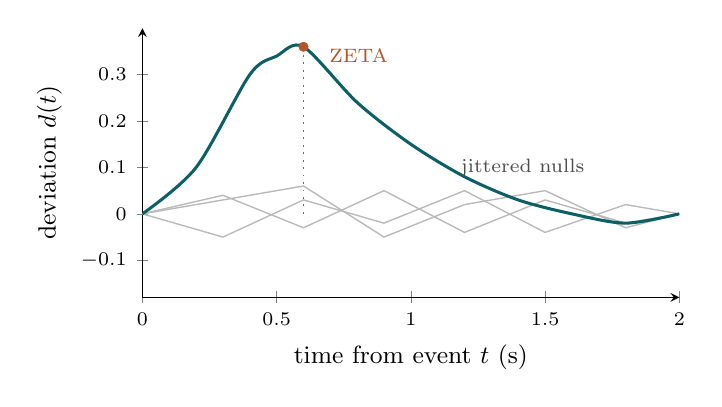
\begin{tikzpicture}
\begin{axis}[
  width=8.4cm, height=5.0cm,
  xlabel={\small time from event $t$ (s)},
  ylabel={\small deviation $d(t)$},
  xmin=0, xmax=2, ymin=-0.18, ymax=0.40,
  xtick={0,0.5,1,1.5,2}, ytick={-0.1,0,0.1,0.2,0.3},
  tick label style={font=\scriptsize}, label style={font=\scriptsize},
  axis lines=left,
]
% null deviation curves (jittered onsets) -- small wiggles near zero
\addplot[gray!55, line width=0.5pt] coordinates {
  (0,0)(0.3,0.04)(0.6,-0.03)(0.9,0.05)(1.2,-0.04)(1.5,0.03)(1.8,-0.02)(2,0)};
\addplot[gray!55, line width=0.5pt] coordinates {
  (0,0)(0.3,-0.05)(0.6,0.03)(0.9,-0.02)(1.2,0.05)(1.5,-0.04)(1.8,0.02)(2,0)};
\addplot[gray!55, line width=0.5pt] coordinates {
  (0,0)(0.3,0.03)(0.6,0.06)(0.9,-0.05)(1.2,0.02)(1.5,0.05)(1.8,-0.03)(2,0)};
% the real deviation curve
\addplot[deepteal, line width=1.1pt, smooth] coordinates {
  (0,0)(0.2,0.10)(0.4,0.30)(0.5,0.34)(0.6,0.36)(0.8,0.24)
  (1.0,0.15)(1.2,0.08)(1.4,0.03)(1.6,0.0)(1.8,-0.02)(2,0)};
% mark the zenith
\addplot[rust, only marks, mark=*, mark size=1.6pt] coordinates {(0.6,0.36)};
\draw[rust, dotted, line width=0.7pt] (axis cs:0.6,0) -- (axis cs:0.6,0.36);
\node[rust, font=\scriptsize, anchor=west] at (axis cs:0.66,0.34) {ZETA};
\node[gray!60!black, font=\scriptsize, anchor=west]
  at (axis cs:1.15,0.10) {jittered nulls};
\end{axis}
\end{tikzpicture}
\end{center}

\noindent
The teal curve is the real deviation; the grey curves are what shuffling
produces. The real zenith towers over the null maxima, so the $p$-value is
small and the neuron counts as responsive. (Both plots here are schematic, to
show the shapes --- not output from a particular cell.)

% ===========================================================================
\section{Reading the output}

The Python \texttt{zetapy.zetatest} returns the pieces above under these names,
all of which appear in our \texttt{scripts/zeta\_reward\_demo.py} figure:

\begin{itemize}
  \item \texttt{vecRealFrac} --- the cumulative fraction $g(t)$, ending at $1$.
  \item \texttt{vecRealFracLinear} --- the constant-rate diagonal $L(t)$.
  \item \texttt{vecRealDeviation} --- the deviation $d(t)$ whose peak is ZETA.
  \item \texttt{dblZETA} --- the rescaled statistic; \texttt{dblP} its $p$-value.
  \item \texttt{dblZETADeviation} --- signed peak ($>0$ excitation, $<0$
        suppression).
  \item \texttt{dblLatencyZETA} --- the time of the peak (response latency).
  \item a smoothed \textbf{instantaneous firing rate} (IFR), obtained from a
        multi-scale derivative of the same spike times, for plotting and for the
        peak-onset latency.
\end{itemize}

A close relative, \texttt{zetatest2}, compares \emph{two} conditions: it builds
a deviation between their two cumulative curves and tests whether \emph{that}
differs from chance. This is the two-sample ZETA we use to ask whether a
response \emph{differs by outcome} (rewarded vs.\ not, gamble vs.\ safe).

% ===========================================================================
\section{What significance does --- and does not --- mean}

ZETA is powerful precisely because it is sensitive: it detects brief, sharp, or
oddly shaped responses that a fixed bin would miss. But that sensitivity has a
flip side worth stating plainly.

\begin{keybox}
A significant one-sample ZETA means only that the neuron's spike timing is
\emph{not flat} around the event --- that \emph{something} time-locked modulates
it. In an awake, behaving task almost every neuron is engaged by \emph{some}
correlate of the event (movement, arousal, attention), so a very high fraction
testing significant is expected. It is a statement about responsiveness, not
about \emph{what} is encoded.
\end{keybox}

\noindent
Two cautions follow. First, the $p$-value measures \emph{detectability}, which
grows with spike and trial count; it is not an effect size. Second, ``responds
to the event'' is a much weaker claim than ``encodes reward'' or ``encodes
choice''. To get at coding you must hold the confounds constant and contrast
conditions --- the two-sample ZETA (\texttt{zeta\_outcome.py}) or a
regression of firing rate on a specific latent variable. The one-sample test
opens the door; the contrasts tell you which room you are in.

% ===========================================================================
\section{Symbol glossary}

\begin{center}
\begin{tabular}{@{}ll@{}}
\toprule
\textbf{Symbol} & \textbf{Meaning} \\
\midrule
$T$            & Analysis window length after the event (\texttt{dblUseMaxDur}; $2$\,s here). \\
$n$            & Total spikes pooled across all trials within $[0,T]$. \\
$t_1\dots t_n$ & Spike times relative to event onset, sorted ascending. \\
$g(t)$         & Cumulative spike fraction (empirical CDF); runs $0\to 1$. \\
$L(t)=t/T$     & Constant-rate baseline: cumulative fraction under no time-locking. \\
$d(t)$         & Temporal deviation $g(t)-L(t)$, mean-subtracted; a Brownian bridge under $H_0$. \\
ZETA           & $\max_t|d(t)|$: the largest temporal departure from constancy. \\
\texttt{dblZETA} & The rescaled ($z$-scored) statistic actually reported. \\
\texttt{dblZETADeviation} & Signed peak: $>0$ excitation, $<0$ suppression. \\
\texttt{dblLatencyZETA}   & Time of the peak deviation --- the response latency. \\
\texttt{intResampNum}     & Number of jittered-onset shuffles building the null. \\
\texttt{zetatest2}        & Two-sample variant: tests whether two conditions differ. \\
\bottomrule
\end{tabular}
\end{center}

\vspace{1.2em}
\begin{keybox}
\textbf{(1)} Spikes become a cumulative fraction that climbs from $0$ to $1$,
erasing firing rate and keeping timing. \textbf{(2)} ZETA is the largest gap
between that curve and the straight line a constant rate would draw.
\textbf{(3)} Its null is the maximum of a Brownian bridge, so a $p$-value falls
out with no bins --- but it certifies \emph{responsiveness}, not \emph{coding}.
\end{keybox}

\end{document}
